%%
%% This is file `sample-xelatex.tex',
%% generated with the docstrip utility.
%%

%% The original source files were:
%%
%% samples.dtx  (with options: `sigconf')
%% 
%% IMPORTANT NOTICE:
%% 
%% For the copyright see the source file.
%% 
%% Any modified versions of this file must be renamed
%% with new filenames distinct from sample-sigconf.tex.
%% 
%% For distribution of the original source see the terms
%% for copying and modification in the file samples.dtx.
%% 
%% This generated file may be distributed as long as the
%% original source files, as listed above, are part of the
%% same distribution. (The sources need not necessarily be
%% in the same archive or directory.)
%%
%% The first command in your LaTeX source must be the \documentclass command.
%\documentclass[sigconf]{acmart}
\documentclass[10pt,conference]{IEEEtran}
%\documentclass[sigconf,review,anonymous]{acmart}

% Copyright 2017 Sergei Tikhomirov, MIT License
% https://github.com/s-tikhomirov/solidity-latex-highlighting/

\usepackage{listings, xcolor}

\definecolor{verylightgray}{rgb}{.97,.97,.97}

\lstdefinelanguage{Solidity}{
	keywords=[1]{anonymous, assembly, assert, balance, break, call, callcode, case, catch, class, constant, continue, constructor, contract, debugger, default, delegatecall, delete, do, else, emit, event, experimental, export, external, false, finally, for, function, gas, if, implements, import, in, indexed, instanceof, interface, internal, is, length, library, log0, log1, log2, log3, log4, memory, modifier, new, payable, pragma, private, protected, public, pure, push, require, return, returns, revert, selfdestruct, send, solidity, storage, struct, suicide, super, switch, then, this, throw, transfer, true, try, typeof, using, value, view, while, with, addmod, ecrecover, keccak256, mulmod, ripemd160, sha256, sha3}, % generic keywords including crypto operations
	keywordstyle=[1]\color{blue}\bfseries,
	keywords=[2]{address, bool, byte, bytes, bytes1, bytes2, bytes3, bytes4, bytes5, bytes6, bytes7, bytes8, bytes9, bytes10, bytes11, bytes12, bytes13, bytes14, bytes15, bytes16, bytes17, bytes18, bytes19, bytes20, bytes21, bytes22, bytes23, bytes24, bytes25, bytes26, bytes27, bytes28, bytes29, bytes30, bytes31, bytes32, enum, int, int8, int16, int24, int32, int40, int48, int56, int64, int72, int80, int88, int96, int104, int112, int120, int128, int136, int144, int152, int160, int168, int176, int184, int192, int200, int208, int216, int224, int232, int240, int248, int256, mapping, string, uint, uint8, uint16, uint24, uint32, uint40, uint48, uint56, uint64, uint72, uint80, uint88, uint96, uint104, uint112, uint120, uint128, uint136, uint144, uint152, uint160, uint168, uint176, uint184, uint192, uint200, uint208, uint216, uint224, uint232, uint240, uint248, uint256, var, void, ether, finney, szabo, wei, days, hours, minutes, seconds, weeks, years},	% types; money and time units
	keywordstyle=[2]\color{teal}\bfseries,
	keywords=[3]{block, blockhash, coinbase, difficulty, gaslimit, number, timestamp, msg, data, gas, sender, sig, value, now, tx, gasprice, origin},	% environment variables
	keywordstyle=[3]\color{violet}\bfseries,
	identifierstyle=\color{black},
	sensitive=false,
	comment=[l]{//},
	morecomment=[s]{/*}{*/},
	commentstyle=\color{gray}\ttfamily,
	stringstyle=\color{red}\ttfamily,
	morestring=[b]',
	morestring=[b]"
}

\lstset{
	language=Solidity,
	backgroundcolor=\color{verylightgray},
	extendedchars=true,
	basicstyle=\footnotesize\ttfamily,
	showstringspaces=false,
	showspaces=false,
	numbers=left,
	numberstyle=\footnotesize,
	numbersep=9pt,
	tabsize=2,
	breaklines=true,
	showtabs=false,
	captionpos=b
}
\usepackage{bera}% optional: just to have a nice mono-spaced font

\colorlet{punct}{red!60!black}
\definecolor{background}{HTML}{EEEEEE}
\definecolor{delim}{RGB}{20,105,176}
\colorlet{numb}{magenta!60!black}

\lstdefinelanguage{json}{
    basicstyle=\normalfont\ttfamily,
    numbers=left,
    numberstyle=\scriptsize,
    stepnumber=1,
    numbersep=8pt,
    showstringspaces=false,
    breaklines=true,
    frame=lines,
    backgroundcolor=\color{background},
    literate=
     *{0}{{{\color{numb}0}}}{1}
      {1}{{{\color{numb}1}}}{1}
      {2}{{{\color{numb}2}}}{1}
      {3}{{{\color{numb}3}}}{1}
      {4}{{{\color{numb}4}}}{1}
      {5}{{{\color{numb}5}}}{1}
      {6}{{{\color{numb}6}}}{1}
      {7}{{{\color{numb}7}}}{1}
      {8}{{{\color{numb}8}}}{1}
      {9}{{{\color{numb}9}}}{1}
      {:}{{{\color{punct}{:}}}}{1}
      {,}{{{\color{punct}{,}}}}{1}
      {\{}{{{\color{delim}{\{}}}}{1}
      {\}}{{{\color{delim}{\}}}}}{1}
      {[}{{{\color{delim}{[}}}}{1}
      {]}{{{\color{delim}{]}}}}{1},
}

\IEEEoverridecommandlockouts
% The preceding line is only needed to identify funding in the first footnote. If that is unneeded, please comment it out.
\usepackage{cite}
\usepackage{amsmath,amssymb,amsfonts}
\usepackage{algorithmic}
\usepackage{graphicx}
\usepackage[numbers]{natbib}
\usepackage{textcomp}
\usepackage{xcolor}
\usepackage{listings}
\usepackage{courier}
\usepackage{xurl}
\usepackage{hyperref}
\usepackage{relsize,xspace}
\usepackage{fancyhdr}%construct and control page headers and footers

\usepackage{listings}
\usepackage{xcolor}

\newcommand{\totalContracts}{26,799\xspace}

\definecolor{codegreen}{rgb}{0,0.6,0}
\definecolor{codegray}{rgb}{0.5,0.5,0.5}
\definecolor{codepurple}{rgb}{0.58,0,0.82}
\definecolor{backcolour}{rgb}{0.95,0.95,0.92}

\lstdefinestyle{mystyle}{
    backgroundcolor=\color{backcolour},   
    commentstyle=\color{codegreen},
    keywordstyle=\color{magenta},
    numberstyle=\tiny\color{codegray},
    stringstyle=\color{codepurple},
    basicstyle=\ttfamily\footnotesize,
    breakatwhitespace=false,         
    breaklines=true,                 
    captionpos=b,                    
    keepspaces=true,                 
    numbers=left,                    
    numbersep=5pt,                  
    showspaces=false,                
    showstringspaces=false,
    showtabs=false,                  
    tabsize=2
}

\lstset{style=mystyle}
%% NOTE that a single column version may be required for 
%% submission and peer review. This can be done by changing
%% the \doucmentclass[...]{acmart} in this template to 
%% \documentclass[manuscript,screen]{acmart}
%% 
%% To ensure 100% compatibility, please check the white list of
%% approved LaTeX packages to be used with the Master Article Template at
%% https://www.acm.org/publications/taps/whitelist-of-latex-packages 
%% before creating your document. The white list page provides 
%% information on how to submit additional LaTeX packages for 
%% review and adoption.
%% Fonts used in the template cannot be substituted; margin 
%% adjustments are not allowed.
%%
%%
%% \BibTeX command to typeset BibTeX logo in the docs
\AtBeginDocument{%
  \providecommand\BibTeX{{%
    \normalfont B\kern-0.5em{\scshape i\kern-0.25em b}\kern-0.8em\TeX}}}


\begin{document}

%%
%% The "title" command has an optional parameter,
%% allowing the author to define a "short title" to be used in page headers.
%\title{Solidity Smart Contracts: Language constructs for control/currency exchange and guards}
\title{An Exploratory Study on Solidity Guards and Ether Exchange Constructs}

% Double blind Workshop - No author information in this version


%\author{
%\IEEEauthorblockN{Darin Verheijke}
%\IEEEauthorblockA{\textit{Department of Computer Science} \\
%\textit{University of Antwerp}\\
%Antwerp, Belgium \\
%darin.verheijke@student.uantwerpen.be}
%\and
%\IEEEauthorblockN{Henrique Rocha}
%\IEEEauthorblockA{\textit{Department of Computer Science} \\
%\textit{Loyola University Maryland}\\
%Baltimore, USA \\
%henrique.rocha@gmail.com}
%}
\author{
\IEEEauthorblockN{Placeholder 1st Author}
\IEEEauthorblockA{\textit{Department 1} \\
\textit{Affiliation 1}\\
City, Country \\
author1@email.com}
\and
\IEEEauthorblockN{Placeholder 2nd Author}
\IEEEauthorblockA{\textit{Department 2} \\
\textit{Affiliation 2}\\
City,  Country \\
author2@email.com}
}


\maketitle

%%
%% The abstract is a short summary of the work to be presented in the
%% article.
\begin{abstract}
Ethereum is a blockchain platform that enables the use of smart contracts. Smart contracts will execute a set of instructions without an intermediary party when called upon. The possibility to make calls to another contract or exchange cryptocurrency allows for potential exploits to occur, most notable reentrancy. The Solidity language for coding smart contracts has syntactic constructs created to be safer alternatives, and guards to aid in securing code against exploits. In this paper, we collect a total of \totalContracts verified Solidity smart contracts from Etherscan, to analyze the language constructs used in calling another contract or exchanging ether. We also analyze the usage of guards to make the code more secure. For instance, even though call is the unsafest function, it is still used by 50\% of the contracts in our dataset. The safe method transfer is used by approximately one-third of contracts, and send is rarely used.

%In this paper we will discuss and look at how one of these exploits, called the reentrancy attack, is possible. This attack is most well known for The DAO attack in 2016 where almost 55 million dollar got drained by an attacker who made use of this vulnerability in the smart contract. More specifically we will look at the concept in the Solidity programming language which was made specifically for the Ethereum blockchain. Also an overview of the different advantages and disadvantages of the different functions to exchange Ether, the currency used to execute transactions, will be given, how they work and how the call function might allow for certain exploits. The reentrancy vulnerability is still prevalent in smart contracts nowadays and forms a huge threat to applications and their users due to the huge possible financial losses that can happen. This research also includes an analysis of a verified smart contract database that was collected from Etherscan. This was done to detect potential vulnerabilities by looking for the presence of functions that allow for these attacks. Finally, the results of this analysis are discussed and there will be a brief discussion about prevention measures and methods to avoid a reentrancy attack.
\end{abstract}

\begin{IEEEkeywords}
Smart Contracts, Solidity,  Call,  Transfer,  Guards.
\end{IEEEkeywords}


\section{Introduction}

A blockchain is an append-only transactional database where the information is structured together in groups, also known as blocks \cite{smart_inspect, smarter}. Each block has certain storage capacities and is chained onto the previous filled block, thus forming a blockchain. Another way to define it is a shared, immutable ledger that records transactions that can be used to track different assets. The most notable uses of this blockchain technology are the cryptocurrencies Bitcoin\cite{article} and Ether \cite{ethereum, white_paper} on the Ethereum network. One important difference between these two blockchain platforms is that Ethereum enables the deployment of smart contracts.

A smart contract is a contract that executes automatically when called upon where the terms between the two parties are written in code (on the blockchain). These contracts then run when a function is called and the conditions for that function are met and can be used to automate executions of agreements without any intermediary party \cite{criminal, 10.1145/2993600.2993611, smarter}. In its simplest form, a contract is just a collection of functions. Interesting to note is that all smart contract transactions are traceable, transparent, and also irreversible \cite{smart_inspect, smarter}.

A common functionality of smart contracts is the possibility to make calls to another contract on the same blockchain platform. This however needs to be done with caution as untrusted contracts can not only introduce errors but also risks as the contract or call may execute malicious code and exploit vulnerabilities. Every call transfers execution control to the called contract.

One of these dangers when calling an external contract is called reentrancy and is one of the most well-known attacks due to the DAO Attack in June 2016 where around 3.6 million Ether was taken which equated to around \$50 million dollar at the time \cite{10.1007/978-3-662-54455-6_8}. This exploit is cemented in the history of Ethereum as it resulted in Ethereum being forked into Ethereum Classic and the Ethereum we know today.
The original version of this attack involved functions that would be called repeatedly before the first function was finished.

Solidity is one of the major programming languages for smart contracts on Ethereum. To avoid these exploits, there have been introduced more language constructs and recommended coding patterns. More specifically, the function call() was to be replaced by the safer functions transfer() and send(). However, recently there has been a switch back to the call() function with the introduction of EIP 1884 \cite{eip1884}. Other precautions instead must be taken to prevent reentrancy attacks, one recommendation is making use of safe code patterns and using guards.

In this paper, we conduct an exploratory research investigating how these calling functions are used in practice and if they are still commonly used for the current smart contracts being deployed in the Ethereum network. For this study, we collected a dataset of \totalContracts unique open-source verified smart contracts from Etherscan (from 2012-07-07 to 2022-01-06). We present different characteristics for the contracts and the Solidity language constructs being used.


\section{Background}
An introduction to some important concepts such as blockchain, the consensus mechanism used in Ethereum, smart contracts and reentrancy attacks is given. The scope of these concepts will be kept to the Ethereum blockchain and one of its programming languages Solidity~\cite{solidity}.

\subsection{Blockchain}
A blockchain is a decentralized, distributed and immutable ledger that differs from a typical database in the way that it stores information. All recorded transactions, structured in blocks, are linked together using cryptography. Each block will contain a hash of the previous block, a timestamp and transaction data. As each block contains information from the previous block due to the hash, they will form a chain, thus forming a blockchain~\cite{article}. It is a peer-to-peer network connecting participants. These participants will be forced to cooperate using a consensus mechanism which enforces rules in order to decentralize control.

\subsection{Consensus mechanisms}
A blockchain reaches consensus when at least 51\% of the nodes on the network agree on the next state of the network. These consensus mechanisms are designed to prevent 51\% attacks on the network. Executing a 51\% attack would require the attacker to have 51\% of the nodes on the network which is considered theoretically impossible due to the decentralized nature of a blockchain but would allow the attacker to decide on the next state of the network by himself due to controlling over half of the nodes and thus choosing which state is correct. Currently, Ethereum uses a proof-of-work consensus mechanism which defines the work that miners (network operators) have to do add a new valid block to the chain. The 'work' they do is a cryptographic math puzzle where the winner (i.e. the fastest to solve the puzzle) earns a reward and shares the new block with the rest of the network. This concept is called 'mining' and has as purpose to secure the blockchain with as incentive newly minted currency of the respective blockchain as a way to reward those who contribute to the system. There has been some criticism on POW due to the amount of energy used and needed to keep the network safe. The Ethereum network consumes 73.2 TWh annually which is comparable to the amount of energy used in Belgium which is 82.16 TWh. Ethereum thus plans to move to proof-of-stake which at a high level has the same end-goal as POW. Very briefly explained, miners will be replaced with validators who can stake their Ether to activate the ability to create new blocks. This consensus mechanism should also have a stronger immunity to centralization as POS should lead to more nodes in the network. For more information on the POS consensus mechanism and Ethereum their change to it we refer to the documentation~\cite{ethereum}~\cite{white_paper}.

\subsection{Ethereum \& Smart contracts}
Ethereum differs from Bitcoin in that it enables the deployment of smart contracts and decentralized applications also known as dApps with built-in economic functions. While bitcoin its primary focus is to be a digital currency payment network, Ethereum is designed to be a general-purpose programmable blockchain that runs a virtual machine capable of executing code.
Ether is the currency used to complete transactions on the network and is used as a way to meter and constrain execution resource costs. In comparison to bitcoin, Ether is designed to be a utility currency which is used to call transactions on the Ethereum platform as a sort of fee~\cite{mastering}. Ethereum has two account types, Externally-owned accounts and contracts. Externally-owned accounts can be controlled by anyone who has the private keys to this account while smart contracts are deployed to the network and are controlled by code.
Smart contracts can be used to create a range of dApps.  An important feature of smart contracts is that when a function is called and the conditions for that function are met there is an automatic execution of the set agreements without any intermediary party~\cite{ethereum, white_paper}.

We take a look at the vending machine example introduced by Nick Szabo, who first coined the term 'Smart contract'~\cite{nick}. A simple vending machine will take in coins and via a simple mechanism dispense change and the output we selected. How a vending machine removes the need for a vendor employee, smart contracts remove the need for an intermediary party. Some important properties of smart contracts is that they are immutable and deterministic. Immutable because once deployed due to the nature of how a blockchain works, the code can not change of the smart contract. The only way to modify a smart contract is to deploy a new instance (and thus a new smart contract). Deterministic in the way the outcome after is identical for everyone who, given the same transaction parameters and state of the Ethereum blockchain, executes the contract ~\cite{white_paper}.

Important to note, contracts are only run if they are called by a transaction. A contract can call another contract that in its turn can then call another contract however the first part of this chain will always be a transaction called by an Externally-owned account. All transactions will either successfully terminate or revert. While a contract can not be changed, it can be deleted, removing the code and its storage from its address leaving an empty account. Any transactions sent there will not result in any execution of code. 

Executing a transaction requires a fee which is called the gas fee. It refers to the amount of computational effort required to execute specific operations, these fees are paid in Ether. It's part of the reward miners get in exchange for their service. Gas prices are denoted in gwei which is equal to $10^{-9}$ Ether. These fees help keep the network secure by preventing bad actors from spamming the network ~\cite{docs}.

Anybody with enough Ether can deploy and write a smart contract to the network. Deployment of a smart contract is also considered a transaction and thus also requires a gas fee.
\subsection{Solidity}

Solidity~\cite{solidity} is one of the main languages to code smart contracts in the Ethereum platform. Solidity is an object-oriented, high-level language that has syntax comparable to C++.

\subsubsection{Solidity Ether Exchange}

We like to highlight the language constructs used to exchange cryptocurrency among contracts: call, send, and transfer (Table~\ref{tab:freq}).

The call function is a low-level interface for sending a message to a contract and it is also a way to send Ether to another address. The call function transfers the execution control to the called contract and the caller can forward any amount of gas. Therefore, the call function has the potential to introduce vulnerabilities, most notably reentrancy.

The transfer method was first introduced in version 0.4.10 (May 2017) of the Solidity language. It provides a safe-by-design method to transfer cryptocurrency. Even though this method also transfers the execution control to the caller, it has a gas limit that prevents abuse. If the transfer fails, an exception is raised, which also adds to the security of this method as the exception reverts the transaction. Due to automatically reverting in case of errors, the transfer function is recommended in most cases.

The send function can be seen as a lower-level implementation of transfer. Similar to transfer, it provides a safe-by-design function to transfer cryptocurrency, with a gas limit to prevent exploits. The major difference between send and transfer, is that send returns false if it fails, delegating the error handling to the developer.


\begin{table}
\center
  \caption{Solidity Functions to Exchange Ether}
  \label{tab:freq}
  \begin{tabular}{ccl}
    \hline
    Function & Gas Limit & Error Handling\\
    \hline
    call & Custom & Returns false on failure\\
    transfer & 2300 & Throws exception on failure\\
    send & 2300 & Returns false on failure\\
  \hline
\end{tabular}
\end{table}

\subsubsection{Solidity Guards}

Guards are language constructs to prevent access or revert a transaction. In Solidity, \textit{Require} and \textit{Assert} have been introduced to the language in the version 0.4.10 (May 2017); \textit{Revert} was introduced in version 0.4.12 (Ago 2017).

Both {require} and {assert}, check for a condition and raise an exception if such condition is not met. Any exception in a smart contract execution will cancel the transaction. Assert is supposed to be a check for internal errors and bugs. Assert will consume all remaining gas. On the other hand, require intent is to be used as much as possible for developers to check for conditions. Require refunds remaining gas if it raises an exception.
%
Revert raises an exception while refunding the remaining gas. It is similar to a "throws new Exception()" in Java.

Those three methods (assert, require, and revert) are guards to stop a transaction and prevent possible exploits in a smart contract. The usage of these constructs may indicate that developers are concerned with the security of the contract.

\subsection{Reentrancy attack}

The call function has some vulnerabilities. Every call to another contract transfers execution control to the called contract. Untrusted contracts may introduce and execute malicious code or exploit vulnerabilities. One of these major vulnerabilities is called the reentrancy attack, which takes advantage of the transfer of execution control by making recursive calls back to the original contract, repeating executions, and creating new transactions.

The two main types of reentrancy attacks are single function and cross-function: Single function, and Cross-function.

\subsubsection{Single function reentrancy attack}
This version repeatedly calls the involved function before the first invocation of the function is finished.  Listing~\ref{lst:reentrancy1} shows a code snipped with this exploit.

\begin{lstlisting}[language=Solidity, caption=Single function reentrancy attack, label=lst:reentrancy1]
mapping (address => uint) private userBalances;

function withdrawBalance() public {
    uint amountToWithdraw = userBalances[msg.sender];
    (bool succes, ) = msg.sender.call.value(amountToWithdraw)("");
    require(success);
    userBalances[msg.sender] = 0;
    }
// Fallback function which gets executed
function () public payable {
    withdrawBalance()
}
\end{lstlisting}

In this example,  an attacker can recursively call the \texttt{withdrawBalance()} function and drain the whole contract as the user's balance is only set to 0 at the very end of the function.

\subsubsection{Cross-function reentrancy attack}
When a function shares a state with another function there is a possibility of a cross-function reentrancy attack.  Listing~\ref{lst:reentrancy2}  shows a code snipped with a cross-function reentrancy vulnerability. 

\begin{lstlisting}[language=Solidity, caption=Cross-function reentrancy attack, label=lst:reentrancy2]
mapping (address => uint) private userBalances;

function transfer(address to, uint amount) {
    if (userBalances[msg.sender] >= amount) {
        userBalances[to] += amount;
        userBalances[msg.sender] -= amount;
        }
    }
function withdrawBalance() public {
    uint amountToWithdraw = userBalances[msg.sender];
    (bool succes, ) = msg.sender.call.value(amountToWithdraw)("");
    require(success);
    userBalances[msg.sender] = 0;
}

\end{lstlisting}

Here the attacker will call the transfer function when the code is executed on an external call in \texttt{withdrawBalance()},  again the user's balance is not yet set to 0 and thus they will be able to transfer tokens again. A simple solution to both these types of attacks is updating the balance before transferring control to another function or contract.  Another simple solution would be to use transfer or send (the safer-by-design constructs) instead of call.

\subsection{Prevention}
In this section we will discuss different patterns and methods to reduce the possibility of attacks and exploits in a smart contract. 

\subsubsection{Checks Effects Interactions pattern}
The goal of this pattern is to reduce the attack surface for malicious contracts who try to hijack control flow after a call. 
As mentioned before, control flow will be transferred to an external contract when calling an external address. In case we have a bad actor, this can cause unexpected behavior and possibly allow the attacker to repeatedly invoke functions that should've been only executed once. The Checks Effects Interactions pattern will update all state variables prior to an external call.~\cite{cei} In other words, the effect is accounted for before completion. This will not cause any issues if anything goes wrong with the contract due to the whole transaction, including the reduction of balance being reverted. An example is given in the code below ~\ref{lst:cei} of the different parts of this pattern, this method was first described in the Solidity documentation~\cite{solidity}. As we can see in the contract, the first step is utilizing a require check in order to make sure that the balance of the user is sufficient. After that the user balance gets reduced which is the effect and all external calls take place after this effect. Notice the use of the transfer function, this propagates every exception that is thrown at the receiving address to the sending contract, which leads to the automatic revert of all changes in the state . The pattern discussed in the next section can be used to include exception propagation for both the send and call function.

\begin{lstlisting}[language=Solidity, caption=Checks Effects Interactions pattern, label={lst:cei}]
contract ChecksEffectsInteractions {
    
    mapping(address => uint) balances; // Stores user balances
    
    function deposit() public payable {
        balances[msg.sender] = msg.value;
        }
    function withdraw(uint amount) public {
        require(balances[msg.sender] >=amount); // Checks
        
        balances[msg.sender] -= amount; // Effects
        
        msg.sender.transfer(amount); // Interactions
    }
}

\end{lstlisting}

\subsubsection{Guard Check pattern}
This pattern can be used to validate user inputs, check the contract state before executing any logic aswell as invariants in the code and rule out any conditions that should not be possible. Triggering exceptions in Solidity is done by using either the revert(), require() or assert() functions. Solidity documentation recommends require() to ensure valid conditions such as inputs, state variables or to validate return values from calls to external contracts ~\cite{solidity}. This should be implemented towards the beginning of the function as a way to validate. Assert() is used to test for internal errors and to check invariants and is used towards the end of a function. Both these functions will evaluate the parameters and throw an exception only if it evaluates to false, the revert() function will throw an exception in each case and is used in more advanced scenarios such as if-else trees. An example of the different guards can be seen in the following code fragment~\ref{lst:guard}where we made a deposit function that only sends money if the user we send too has a balance less than us~\cite{guardcheck}. 


\begin{lstlisting}[language=Solidity, caption=Guard Check pattern, label={lst:guard}]
contract GuardCheck {
     function deposit(address addr) payable public {
        require(addr != address(0)); // Ensures address is not 0 and that the user has specified an address to deposit too
        require(msg.value !=0 ); // Ensures that their is a value attached to the transaction, else we stop right here
        
        uint balanceBeforeTransfer = this.balance;
        uint transferAmount;
        
        if (addr.balance < msg.sender.balance) {
            transferAmount = msg.value;
        }
        else {
            revert(); // We only send money if the address we want to send too has less money than us
        }
        
        addr.transfer(transferAmount);
        assert(this.balance == balanceBeforeTransfer - transferAmount); // Makes sure that the current balance after the deposit is equal to the balance before minus the deposited amount. 
     }
     
}
\end{lstlisting}

\subsubsection{Mutex}
Another way of protecting the state of a contract is by adding a mutex. This will be especially handy with dealing with cross-function reentrancy attacks. The concept will be to protect pieces of code where shared resources are accessed. To utilize these resources the mutex will first need to be unlocked as it will only be possible for the resource to be changed by one process or function at a time. A simple implementation of utilizing a mutex is given in code sample below ~\ref{lst:mutex}. The mutex variable makes exploit of a recursive call impossible and also avoids a cross-function reentrancy attack. Note that it is important to ensure a way for a lock to be released as a contract without release of its lock can be rendered inert. 

\begin{lstlisting}[language=Solidity, caption=Mutual exclusion, label={lst:mutex}]

contract Mutex {
    mapping(address => uint) balances; // Stores user balances

    function transfer(address to, uint amount) external {
        require(!lock);
        lock = true;
        
        if (balances[msg.sender] >= amount) {
            balances[to] += amount;
            balances[msg.sender] -= amount;
        }
        lock = false;
    }
    function withdraw() external {
        require (!lock);
        lock = true;
        uint amount = balances[msg.sender];
        require(msg.sender.call.value(amount)());
        balances[msg.sender] = 0;
    }
    lock = false;
}
\end{lstlisting}
\subsection{The DAO attack}
The most well known real-world example of such a reentrancy attack was 'The DAO Hack'. We will briefly discuss this attack as it shows the significance and importance of preventing reentrancy attacks.
\subsubsection{The DAO}
 DAO stands for "Decentralized Autonomous Organization". In other words, the organization is not run by any institution but instead will run automatically based on pre-defined smart contracts. All transactions and rules are thus encoded on the blockchain. The purpose of The DAO was to be a governance model for crowd investments. All members would send a certain amount of Ether to the DAO after which members of the DAO could make proposals for investments and then vote on those proposals. Other interesting realized concepts of DAOs are Constitution DAO \cite{constitution}, an organisation that tried to purchase an original copy of the US constitution, CityDAO, a project that is trying to create entirely new cities from scratch, governed by a DAO~\cite{citydao}~\cite{cryptocities} and KlimaDAO, where the collective has the goal of accelerating price appreciation of carbon assets and earns rewards based on climate action~\cite{klimadao}. 
 An important part of the governance model of The DAO was the split functionality in which it was possible for users to create a proposal to split from the DAO where the user takes their stake from the contract and splits from the DAO into a child DAO thus leaving The DAO and burning their ownership of the current one. After a fixed period of time, it was possible to then retrieve your Ether from that child DAO. 
 
\subsubsection{The attack}
An attacker made use of this split functionality in order to execute a reentrancy attack. The attacker managed to recursively call the functionality which allows to drain your Ether before splitting of in a child DAO due to the internal states not updating before the transfer of the Ether to the child DAO. They were able to drain around 55 out of the 152 million dollars that was crowdfunded before some white hackers managed to create a split themselves and save the remaining Ether. 

\subsubsection{The aftermath}
There were now two child DAO's which controlled the funds but were still time-locked to withdraw their Ether. A decision was made by the Ethereum community to hard fork the Ethereum Blockchain before this funds were freed, essentially going back in time to a version of Ethereum where the DAO attack never happened. This did cause some controversy which is the reason for the existence of both Ethereum Classic and Ethereum nowadays in which Ethereum Classic is the original version in which the DAO attack was not removed.

\subsubsection{Other notable attacks}
More recent examples of reentrancy attacks are the uniswap/lendf.me hacks where 25 million dollar got drained in April of 2020~\cite{lendf}, cream finance hack in August of 2021 where 18.8 million dollar was stolen by exploiting a reentrancy vulnerability that allowed two borrows while doing a flash loan~\cite{cream}.
\section{Study Design}
\subsection{Dataset}

We collected verified smart contracts from Etherscan\footnote{\url{etherscan.io/contractsVerified}} which is a block explorer and analytic platform for Ethereum. Etherscan verified contracts allows the public to audit and read contracts as it has to be made publicly available to be granted the verified status. Etherscan does not give access to a complete dataset of verified smart contracts but rather has an open-source database of the latest 10,000-5,000 smart contracts that were verified. Therefore, we gathered the latest contracts from time to time, over a period of six months (2021-07-07 to 2022-01-06) to build our dataset.

Then, we did the following pre-processing steps in our dataset: (i) remove all duplicated\footnote{We removed contracts with the same address in the Ethereum blockchain. We did not verify whether the contracts with the same name have the same source code. Since these contracts have different addresses, they are considered separate entities in the blockchain platform.} contracts; (ii) remove contracts not written in Solidity; (iii) removed contracts which we could not process using cloc.\footnote{cloc is a tool to count lines of code available at <\url{https://github.com/AlDanial/cloc}>.} After removing those contracts, we had a total of \totalContracts unique verified solidity smart contracts. This dataset is publicly available.\footnote{\url{https://bit.ly/3fyOgBD}, the link has been properly anonymized for the reviewers to download the dataset spreadsheet with the name and address of the contracts and not break the double-blind review process.}


\subsection{Method}

We use the Etherscan API~\cite{etherscan_api} to retrieve the source codes for each contract in our dataset. Listing~\ref{lst:api} shows an example of the API call used to acquire the contract source code.
\begin{lstlisting}[language=solidity, caption=Etherscan API call, label={lst:api}]
https://api.etherscan.io/api?module=contract
&action=getsourcecode
&address=0xb4e32b964f6ae78 //The contract address
&apikey=YourApiKeyToken // Your API key
\end{lstlisting}

Then, we used the cloc tool on the contracts to discover how many lines of code are in each one. We removed from this study the contracts that cloc were not able to process. Moreover, we used a Python script on the contracts to locate specific methods used in the contracts related to Ether exchange functions (call, send, and transfer) and guards (require, assert, revert).

\section{Analysis and Results}

\subsection{Overall Analysis}

First, we show some general characteristics of our dataset.
Table~\ref{tab:loc} shows the general statistics considering the lines of code on the contract. We can see that the contracts in our dataset are small in lines of codes, with a median of 256 LoC and an average of 356 LoC. That is expected, as smart contract code tends to be smaller when compared to software code in other domains.  The smallest contracts have only 2 LoC.  For example, the contract \textit{BlackHole}\footnote{\url{https://etherscan.io/address/0x727E9A3067DeEaF031916fA0fC53B02cf44F8731\#code}} only has two lines, a pragma definition for the solidity version, and an empty contract definition. The biggest contract is \textit{RewardControl}\footnote{\url{https://etherscan.io/address/0xcf8Fe5bB819359Ea02DF65E50B6194D12b69aB88\#code}} with 6,461 LoC. 

\begin{table}
\center
  \caption{Lines of Code (LoC)}
  \label{tab:loc}
  \begin{tabular}{c c c c c}
    \hline
    Min & Median & Average & Std. Dev. & Max \\
    \hline
   2 & 256 & 359 & 335 & 6,461 \\
  \hline
\end{tabular}
\end{table}

Now, we investigate how many Ether exchange methods and guards are being used in the contracts. Table~\ref{tab:results-all} shows how many contracts in our dataset have at least one of the methods, the overall count of the method, and the average number in the contracts that have at least one. Even though call is the unsafest method for Ether exchange, it is used by 50\% of the contracts in the dataset. On average, there are 2.3 call uses on the contracts. Any contract using call has the potential to have a reentrancy vulnerability. On the other hand, send is a safer method and it is the least used (2\%). Transfer is the safest method, and it is used by roughly one-third of contracts.

\begin{table}
\center
  \caption{Ether Exchange and Guards Usage}
  \label{tab:results-all}
  \begin{tabular}{crrr}
    \hline
    Method & Contracts & Count & Average \\
    \hline
    Call & 13,443 (50\%) & 32,236 & 2.3 \\
    Transfer & 9,176 (34\%) & 17,814 & 1.9 \\
    Send & 647 (02\%) & 1,059& 1.6 \\
    Require & 26,190 (97\%) & 622,679 & 23.7 \\
    Assert & 7,279 (27\%) & 10,507 & 1.4 \\
    Revert & 13,819 (51\%) & 41,502 & 3.0\\
    \hline
\end{tabular}
\end{table}

On the guard methods shown in Table~\ref{tab:results-all}, require is used by the great majority of all contracts (97\%). On average, there are 23.7 uses of require in the contracts. The great usage of this guard may be to counteract the vulnerabilities of call. Revert is also commonly used by more than half of the contracts in our dataset. Finally, Assert is the least used guard in our analysis.

\subsection{Contracts by Version}

Table~\ref{tab:major-versions} shows the contracts categorized by their major Solidity version, and the average and median size in lines of code (LoC). Most contracts are from the latest Solidity version, 0.8.x. The oldest Solidity version to appear in our dataset is 0.4.x which has fewer amount of contracts. The biggest average and median LoC size are from contracts of version 0.6.x.

\begin{table}
\center
  \caption{Solidity Major Versions}
  \label{tab:major-versions}
  \begin{tabular}{crrr}
    \hline
    Version & Contracts & Average LoC & Median LoC \\
    \hline
    0.8.x & 14,869 (55\%) & 355 & 285 \\
    0.7.x & 2,454 (09\%) & 432 & 321 \\
    0.6.x & 5,838 (21\%) & 433 & 330 \\
    0.5.x & 2,954 (11\%) & 200 & 121 \\
    0.4.x & 684  (02\%) & 225 & 108 \\
  \hline
\end{tabular}
\end{table}

Figure~\ref{fig:minor-versions} shows the top-10 solidity versions (major and minor) in our contracts. The versions with most contracts are 0.8.4 (18.7\%), 0.6.12 (17.1\%), and 0.8.7 (15.3\%). Together these three versions compose over 50\% of the contracts in our dataset.

\begin{figure}[h]
  \centering
  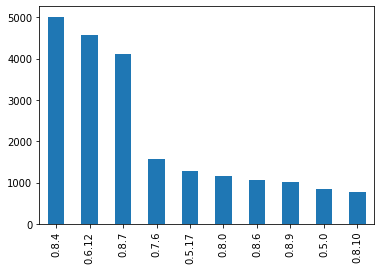
\includegraphics[width=\linewidth]{img/versions_clean.png}
  \caption{Top-10 Solidity versions in the database.}
  %\description{Solidity Compiler Version}
  \label{fig:minor-versions}
\end{figure}

\begin{table}
\center
  \caption{Contracts using Ether Exchange \& Guards by Major Version}
  \label{tab:results-version}
  \begin{tabular}{crrrrrr}
    \hline
      & Call & Send & Transfer & Require & Assert & Revert \\
    \hline
    all & 50\% & 2\% & 34\% &  97\% & 27\% & 51\% \\
    0.8.x & 44\% & 3\% & 33\%  & 98\% & 8\% & 45\% \\
    0.7.x & 67\% & 1\% & 42\% & 98\% & 32\% & 66\% \\ 
    0.6.x & 79\% & <1\% & 32\% & 98\% & 68\% & 79\% \\
    0.5.x & 16\% & <1\% & 29\% & 96\% & 32\% & 20\% \\
    0.4.x & 8\% & 3\%  & 48\% & 92\% & 51\% & 39\% \\
    \hline
\end{tabular}
\end{table}

In Table~\ref{tab:results-version}, we assess the percentage of contracts using at least one of the methods (Call, Send, Transfer, Require, Assert, and Revert) per major version of Solidity. We also included the percentage considering all contracts for comparison.  As we can see, the major version appears to have an impact on the usage of call, transfer, assert, and revert. For instance, versions 0.7.x and 0.6.x have a higher percentage of contracts using call than the normal, and versions 0.5.x and 0.4.x have a lower percentage.  Considering the transfer method,  version 0.7.x and 0.4.x show a higher percentage of contracts using transfer.  

For the guards in Table~\ref{tab:results-version},  versions 0.8.x and 0.5.x show lower percentages for asserts and reverts.  On the other hand, versions 0.7.x and 0.6.x show a higher percentage than normal for the same guard methods. Version 0.4.x shows an increase in contracts using assert but a decrease in contracts using revert. 


\subsection{Contracts using Call}

We focus only on the contracts that contain a call function. Since call is a very unsafe function, there is the possibility for the contracts using it to suffer from a reentrancy vulnerability. For this reason, such contracts may have different characteristics. Table~\ref{tab:call-loc} shows the lines of code considering only the contracts that contain a call function. The average and median LoC values are higher than the ones for all contracts. Therefore, the contract with call in our dataset usually has more lines of code. The call contract with the least lines of code is called \textit{FlashBotLowGas}.\footnote{\url{https://etherscan.io/address/0x90ab9a926a1593992547e0f9a0df6401f10421cd\#code}}

\begin{table}[h]
\center
  \caption{Contracts using Call - Lines of Code}
  \label{tab:call-loc}
  \begin{tabular}{c c c c c}
    \hline
    Min & Median & Average & Std. Dev. & Max \\
    \hline
   6 & 530 & 511 & 367 & 5,572 \\
  \hline
\end{tabular}
\end{table}

Figure~\ref{fig:call_version} shows the Solidity versions for contracts with call. The version with most contracts using call is 0.6.12.  The top-3 versions for all contracts are also the top-3 for contracts with call but in different positions. 

\begin{figure}[h]
  \centering
  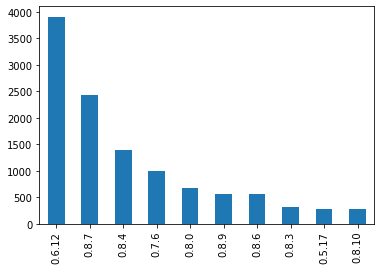
\includegraphics[width=\linewidth]{img/call_clean_v2.png}
  \caption{Top-10 Solidity versions on Contracts using Call. }
  %\description{Solidity Compiler Version}
  \label{fig:call_version}
\end{figure}

Table~\ref{tab:call} show the Ether exchange and guard methods considering only the 13,443 contracts that contain at least one call method. We can see that approximately one-third of the contracts using call also use the send function. We also like to highlight that there is a greater number of contracts with call-using guards. For instance, 99\% of the call contracts used Require compared to 97\% of all contracts; 39\% of the call contracts used Assert compared to 27\% of all contracts; and 89\% of the call contracts used Revert compared to 51\% of all contracts. The higher usage of guards is probably to counter the vulnerabilities of call. This may be an indication that Solidity developers are concerned about the security of their contracts especially when using unsafe methods such as call.

\begin{table}
\center
  \caption{Solidity Methods of Contracts using Call}
  \label{tab:call}
  \begin{tabular}{crrr}
    \hline
    Method & Contracts & Count & Average\\
    \hline
    Transfer & 4,514 (33\%) & 8,789 & 0.65\\
    Send &582 (04\%) & 920 & 0.07\\
    Require &13,392 (99\%) & 456,461 & 33.96 \\
    Assert & 5,348 (39\%) & 6,701 & 0.49\\
    Revert & 11,976 (89\%) & 38,273 & 2.84\\
\end{tabular}
\end{table}

\subsection{Contracts using Transfer}

Now, we focus only on the contracts that contain a transfer function. Transfer is a much safer alternative than call for Ether exchange. Therefore, we expect the contracts using transfer to have different characteristics than the ones using call.

Table~\ref{tab:transfer-loc} shows the lines of code only from contracts with a transfer function. The median, average, and standard deviation are higher than the ones when considering all contracts. However, the same statistics are lower when compared to the contracts with call. This means that contracts using transfer tend to have lower LoC than the contracts using call. The reason for this difference could be that call will need extra code to protect against vulnerabilities. Since transfer is a safe-by-design function, it will not need as much extra code as call for a more secure contract. The smallest LoC contract using transfer is \textit{TransferValueToMinerCoinbase}\footnote{\url{https://etherscan.io/address/0x8512a66d249e3b51000b772047c8545ad010f27c\#code}} with 6 LoC.

\begin{table}[t]
\center
  \caption{Contracts using Transfer - Lines of Code}
  \label{tab:transfer-loc}
  \begin{tabular}{c c c c c}
    \hline
    Min & Median & Average & Std. Dev. & Max \\
    \hline
   6 & 345 & 452 & 373 & 6,461 \\
  \hline
\end{tabular}
\end{table}

Figure~\ref{fig:transfer_version} shows the solidity versions for contracts that contain transfer.  The top-5 versions for contracts using send are the same top-5 versions for all contracts in our dataset.  This could indicate that the contracts with send may represent a general set similar to all contracts in our dataset.

\begin{figure}[h]
  \centering
  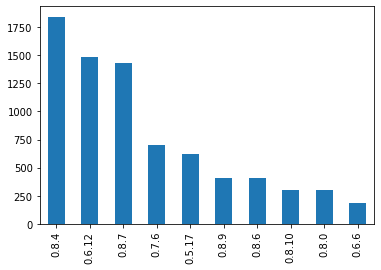
\includegraphics[width=\linewidth]{img/send_versions_clean.png}
  \caption{Top-10 Solidity versions on Contracts using Transfer.}
  %\description{Solidity Compiler Version (Sends)}
  \label{fig:transfer_version}
\end{figure}

\begin{table}
\center
  \caption{Solidity Methods of Contracts using Transfer}
  \label{tab:transfer}
  \begin{tabular}{crrr}
    \hline
    Methods & Contracts & Count & Average \\
    \hline
    Call & 4,514 (49\%) & 11,083 & 1.20\\
    Send &107 (01\%) & 251 & 0.03\\
    Require & 9,060 (98\%) &256,835 & 27.99\\
    Assert & 2,722 (29\%) & 4,789 & 0.52\\
    Revert & 4,876 (53\%) & 14,493 & 1.57 \\
    \hline
\end{tabular}
\end{table}


Table~\ref{tab:transfer} shows the Ether exchange and guard methods considering only the 9,176 contracts that contain at least one transfer method. The percentage of contracts when looking at only contracts with transfer is similar (with a 1-2\% difference) from the ones considering all contracts. This is different from the contracts with call where the guards' percentage increases by a noticeable amount for Assert and Revert.


\subsection{Contracts with Send}

We analyze only the contracts using at least one send method. In our dataset, send is the least used method, being present in only 647 (approximately 2\%) of the contracts. Even though there are fewer contracts to analyze, we expect to obverse different characteristics.

Table~\ref{tab:send-loc} shows lines of code for contracts with send. The median, average, and standard deviation are the highest when compared to all contracts, contracts using call, and contracts using transfer. 
The contract \textit{PaymentManager}\footnote{\url{https://etherscan.io/address/0xaddeb5dbdc1c62c2a2a8e04fddd42e3c3f19587b\#code}} has 2 send functions and it is smallest contract with 15 LoC.

\begin{table}
\center
  \caption{Contracts using Send - Lines of Code}
  \label{tab:send-loc}
  \begin{tabular}{c c c c c}
    \hline
    Min & Median & Average & Std. Dev. & Max \\
    \hline
   15 & 575 & 635 & 498 & 6,461 \\
  \hline
\end{tabular}
\end{table}

The most common Solidity versions for contracts using send were 0.8.7,  0.8.4,  0.8.0,  0.8.10,  and 0.8.6. As we can see,  the top-5 versions are all 0.8.x. 

%\begin{figure}[h]
%  \centering
%  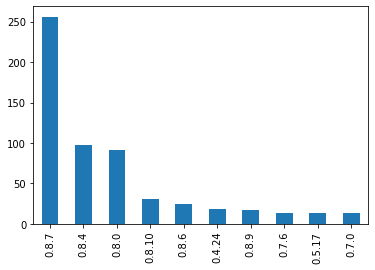
\includegraphics[width=\linewidth]{img/transfer_versions_clean.png}
%  \caption{Top-10 Solidity versions on Contracts using Send.}
%  \label{fig:send_version}
%\end{figure}

Table~\ref{tab:send} show the Ether exchange and guard methods considering only the 647 contracts that contain at least one send function. The contracts percentage are different when contrasted with all contracts. For instance, 89\% of send contracts have a call function compared to 50\% of all contracts; 90\% of send contracts have at least one revert compared to 51\% of all contracts; and in the opposite direction, 16\% of send contracts have at least one transfer method compared to 34\% of all contracts.

\begin{table}
\center
  \caption{Solidity Methods of Contracts using Send}
  \label{tab:send}
  \begin{tabular}{crrr}
    \hline
    Method & Contracts & Count & Average \\
    \hline
    Call& 582 (89\%) & 1,203 & 1.86\\
    Transfer& 107 (16\%) & 234 & 0.36\\
    Require& 647 (100\%) & 25,058 & 38.73\\
    Assert& 63 (09\%) & 166 & 0.26\\
    Revert& 588 (90\%) & 2304 & 3.56\\
    \hline
\end{tabular}
\end{table}

\subsection{Contracts with a Reentrancy vulnerability}
As a last analysis we will take a look at reentrancy vulnerabilities in contracts that contain a call function. The tool slither~\cite{slither} will be used to complete this task and detect the reentrancies in these contracts.
A total of 1,190 reentrancy vulnerabilities were found in a total of 13,443 contracts that contained a call function. In table~\ref{tab:re-loc} we can see that even a contract of only 11 lines of code can contain a reentrancy vulnerability. We have an average of 0.19 reentrancy vulnerabilities per contract when looking at the collection of contracts with this call functionality. A contract called 
 \textit{PostExperiationIdentifierTransformationFinancialProductLibrary}\footnote{\url{https://etherscan.io/address/0xAb955711ECd766Ce70dc2DbF2D9e0E8e4b431232#code}} even contained 38 reentrancy vulnerabilties. The reentrancy vulnerability is thus still prevalent in contracts using a call value function up until this day. 

\begin{table}
\center
  \caption{Contracts with Reentrancies - Lines of Code}
  \label{tab:re-loc}
  \begin{tabular}{c c c c c}
    \hline
    Min & Median & Average & Std. Dev. & Max \\
    \hline
   11 & 639 & 672 & 530 & 5,225 \\
  \hline
\end{tabular}
\end{table}

\section{Related work}


Juels, Kosba and Shi\cite{criminal} investigate the risk of smart contracts fueling new criminal ecosystems. They show how a Criminal Smart Contract can facilitate leakage of confidential information, theft of cryptographic keys, and more, showing the urgency of creating safeguards against these CSCs. They look at questions like how practical these new crimes will be, whether these CSCs enable a wider range of new crimes in comparison to earlier cryptocurrencies such as Bitcoin, and what advantages they offer to criminals in comparison with the conventional online systems.


Luu et al.  \cite{smarter} also investigate and introduce several security problems to manipulate smart contracts in an attempt to gain profit and propose ways to enhance the operational semantics of Ethereum. A focus is put on the semantic gap between the assumption contract writers make about the underlying execution semantics and the actual semantics of the contract are made as a reason for these security flaws. A tool OYENTE is also provided to detect bugs which is a symbolic execution tool. The model works directly with Ethereum virtual machine byte code and thus does not have a need for a higher level representation such as Solidity. An evaluation of OYENTE on 19,366 smart contracts is given where 8,333 contracts were documented as potentially having bugs.

Mense and Flatscher \cite{security} summarize known vulnerabilities found by literature research and analysis such as external calls, gasless sends, mishandled exceptions, and reentrancy. They also compare code analysis tools for their ability to identify vulnerabilities in smart contracts based on a taxonomy for vulnerabilities. The results of their paper show that reentrancy ranks the highest among the vulnerabilities that they have discussed and is detected by most of the tools used. They then delve deeper into the DAO hack as well.


Liu et al. \cite{reguard} present ReGuard which is a fuzzing-based analyzer to automatically detect reentrancy bugs in Ethereum smart contracts. They iteratively generate random (but diverse) transactions, this is called fuzz testing. Then based on the runtime they will identify reentrancy vulnerabilities in a contract. How the architecture works is they parse a smart contracts source or binary code to an intermediate representation which will then be transformed to C++, keeping the original behavior. Together with a runtime library, ReGuard executes the contract and runs an analysis of the operations for any reentrancy attacks.


SmartCheck is an extensible static analysis tool to detect code issues in Solidity by Tikhomirov et al.\cite{smartcheck} where they translate Solidity into an XML-based representation and check it against XPath patterns. They also used a real-world dataset to evaluate their tool and also make a comparison to the earlier mentioned Oyente.


Samreen and Alalfi \cite{survey} explain eight vulnerabilities by looking at past exploitation case scenarios and reviewing some of the available tools and applications to detect these vulnerabilities. For each case they discuss the vulnerability exploited, the tactic used as well as the financial loss that happened. Coverage is given of some preventive techniques as protection against some of these exploits. The tools/frameworks they discuss adopt either a form of static analysis such as symbolic execution and control flow graph construction or dynamic analysis such as the fuzzing testing or tracing the sequence of instructions that are executed at run time.

Tantikul and Ngamsuriyaroj \cite{icissp20} investigate a more recent state of the vulnerabilities of smart contracts. Their research consists of going through a database of verified smart contracts and checking common occurrences as well as trends of vulnerabilities. An analysis is done using both Oyente and Smartcheck and common characteristics of vulnerable smart contracts are identified. A correlation computation is done via Pearson's correlation in order to detect how often any pair of vulnerabilities will be found on the same smart contract. Their results show that overflow and underflow have the highest correlation. Another relation found is the timestamp dependency and transaction ordering which might be caused by malicious miners.  

Bragagnolo et al.~\cite{rocha} address the lack of inspectability of a deployed smart contract. They do this by analyzing the state of the contract using different decompilation techniques. Their solution SmartInspect is an inspector based on pluggable property reflection. Their approach of utilizing mirrors generated from an analysis of Solidity source code allows access to unstructured information from a deployed smart contract in a structured way. This can be done without a need to redeploy or develop additional code for decoding.

Wang et al. \cite{contractward} evaluate a set of real-world smart contracts with ContractWard which uses machine learning techniques to detect vulnerabilities in smart contracts. Their idea was proposed due to existing detection methods being mainly based on symbolic execution or analysis which are very time-consuming. The system extracts dimensional bigram features from simplified operation codes to construct a feature space and can get a predictive recall and precision of over 96\% based on their dataset of 49502 smart contracts on 6 vulnerabilities.

A deep-learning-based approach is used by Qian et al. \cite{automated}. The aim is to precisely detect reentrancy bugs using a bidirectional long-short term memory with an attention mechanism. They also propose using a contract snippet as another way to represent a smart contract only capturing key semantic sentences which contain related and critical information such as control flow and data dependencies. These are then used as input to the sequential models. They show that this deep-learning approach outperforms other state-of-the-art smart contract vulnerability tools.

Slither by Feist et al. \cite{slither} is a static analysis framework that converts Solidity smart contracts into an intermediate representation which they call SlithIR. Static Single Assignment forms are used as well as a reduced instruction set for ease of implementation. Their framework has use cases in automated detection of vulnerabilities, detection of code optimization opportunities, improvement of clarity and ease of understanding of the contracts. An evaluation of the proposed frameworks capabilities is done using a set of real-world smart contracts. 

\section{Final Remarks}

In this paper, we conducted an exploratory study on the usage of specific Solidity language constructs in a dataset of \totalContracts contracts. Even though, call is the unsafest method for Ether exchange it is the most popular method being used by 50\% of contracts. Perhaps because call can be used to transfer the execution control to another contract, and not only for ether exchange, is the reason for its popularity despite the fact that it is unsafe. The other methods for ether exchange, transfer is used by 34\% of contracts, and send is rarely used (2\% of the contracts).

The most popular Solidity versions in our dataset were 0.8.4 (18.7\% of the contracts), 0.6.12 (17.1\% of the contracts), and 0.8.7 (15.3\% of the contracts). We also saw that the usage of call, transfer, assert, and revert can vary a lot from different versions of the contract.

When we focused on only contracts using call, the average and median size in LoC of the contracts are higher than normal. We also noticed an increased percentage of call contracts using more guard methods.

A reentrancy check on the contracts containing the vulnerable call functionality using the tool Slither showed us that reentrancy vulnerabilities are still present in contracts even to this date.  

As future work, we plan to execute more vulnerability detection tools to further investigate the characteristics of the contracts in our dataset.


%%
%% The next two lines define the bibliography style to be used, and
%% the bibliography file.

\bibliographystyle{IEEEtranN}
\bibliography{references}

%\endinput
\end{document}

